\label{chpt:implementation}

This chapter describes the implementation of the task-based 
communication-avoiding ray tracing algorithm designed in 
Chapter~\ref{chpt:design}. The system is implemented using the Intel 
implementation of CnC and is integrated with Embree.  Both libraries are 
introduced in Chapter~\ref{chpt:introduction} and described in
Chapter~\ref{chpt:previous-work}. We start with an overview of the CnC
specification file and then describe implementation details for the CnC tag,
data and step collections.

\begin{figure}[!htb]
  \centering
  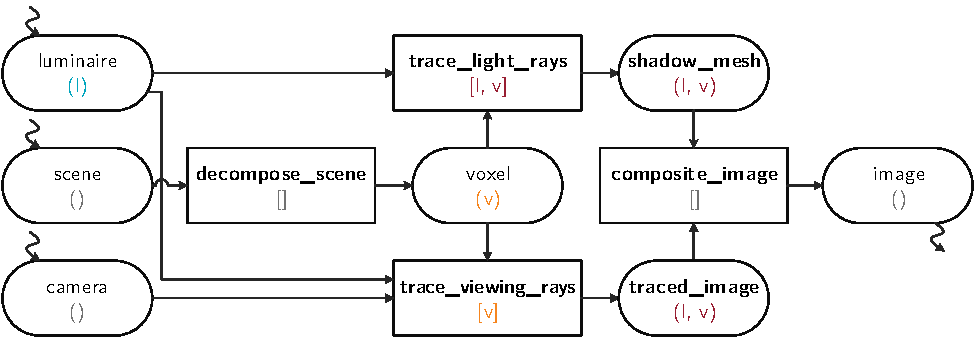
\includegraphics[width=\textwidth]{drawings/CnC.pdf}
  \caption{CnC Graph}
  \label{fig:cnc}
\end{figure}

Figure~\ref{fig:cnc} shows a graphical subset of the full CnC specification (a
full textual version can be found in Figure~\ref{fig:cnc-graph-text}).  Step 
collections are represented as rectangles and data collections are represented
with ovals.  The tag collections are shown in the shape and surrounded with 
either square brackets or parenthesis depending on whether the tag collection is 
within a step collection or a data collection, respectively.  The colors are 
used to group the similar tag collections. The control collection is not 
represented in the graph but can be seen in the textual version. The graph 
begins execution when the object, luminaire, and camera information are
provided, and terminates when an image is produced.

\section{CnC Tag Collections}
\label{sec:tag-collections}
The elements of the tags in the tag collections used in the CnC specification
are \textbf{l} and \textbf{v}.  The \textbf{l} element is an index for a
specific luminaire.  The \textbf{v} element is the index of a specific voxel.
The tag collections, made up of sets of the tag elements, are 
\textbf{\{l\}}, \textbf{\{v\}}, and \textbf{\{l, v\}}.

\section{CnC Data Collections}
\label{sec:data-collections}
\begin{description}
\item[Scene] contains geometry and material information
for the scene being traced and comes from the environment.  In our 
implementation, this information is extracted from WaveFront
``.obj''~\cite{manual-wavefront} files.  A single scene is contained in the
collection for each image to trace.
\item[Camera] contains the location, direction, and field 
of view of the camera in addition to the resolution of the desired output image.
One entry for the camera is contained in the collection for each image to 
trace.
\item[Luminaire] contains information pertaining to each luminaire, including
the type of luminaire, location, direction when applicable, and the desired
number of generated light rays.  The current implementation supports point
and directional luminaires.  Each luminaire is indexed in the collection with a
unique identifier \emph{l}.
\item[Voxel] contains a subset of the geometry and 
material information from the \textbf{scene} data collection.  The subset is 
the information that pertains to the voxel it represents, indexed with the 
\emph{v} element of the collections tag.
\item[Shadow Mesh]contains a boolean value for each 
light ray associated with the indexed \emph{l}.  The collection contains an 
entry for each combination of \emph{l} and \emph{v}, 
\item[Traced Image] contains an array of illumination information and
intersection points for the indexed \emph{l}, \emph{v}.
\item[Image] contains the final composited image, the 
available formats of the output image are those supported by Embree. 
\end{description}

\section{CnC Step Collections}
\label{sec:implementation-step-collections}
\begin{description}
\item[Decompose Scene]reads a ``.obj'' file and produces 
subsets of the scene based on the voxel decomposition.  The number of voxels 
generated is determined by a command line argument and should be more than the 
number of nodes available.  Pseudocode can be found in 
Figure~\ref{fig:decompose-scene}.  The code implemented supports quad and 
triangle geometry as well as materials.  As Embree does not support 
textures, any material using a texture is modified to use a solid color.  
\item[Trace Light Rays] traces the light rays for a single luminaire 
and a single voxel.  Pseudocode for this step can be found in 
Figure~\ref{fig:trace-light-rays}.  Embree is used to determine if the light 
rays intersect any object within the voxel. The light rays are generated by
computing a uniform mesh along the bounding walls of the scene.  Each light ray
points towards a vertex on the mesh.  Light rays for point luminaires
originate from the origin of the luminaire.  Rays from directional luminaires do
not have an origin.  The number of light rays used is a parameter.
\item[Trace Viewing Rays] traces the voxel specified by the 
tag of the step instance using viewing rays generated by Embree based on the
camera information.  Pseudocode for this step can be found in
Figure~\ref{fig:trace-viewing-rays}.  Embree is used to determine if the
viewing rays intersect objects within the voxel.  The helper method referenced
in the pseudocode, \emph{illuminate}, is implemented using an ambient shading
model and a Blinn-Phong Shading model, respectively.  
\newpage
The shading models are implemented as follows:

$$ L^{ambient} = k^a L_a, $$
$$ L^{luminaire} = k^d ( \hat{s_i} \cdot \hat{n}) +
k^s ( \hat{s_i} \cdot \hat{h} )^{n_s} $$

\noindent where $L^{ambient}$ is the ambient radiance, $L^{luminaire}$ is the
luminaire's radiance, $k^a$ is the ambient reflectivity, $L_a$ is the ambient
irradiance, $k^d$ is the diffuse reflectivity, $\hat{s_i}$ is the direction
towards the luminaire, $\hat{n}$ is the surface normal, $k^s$ is the specular
reflectivity, $\hat{h}$ is the halfway vector and $n_s$ is the specular
exponent~\cite{cpts548}.

\item[Composite Image] produces a file containing the final ray traced image. 
Pseudocode can be found in Figure~\ref{fig:composite-image}.  The format of the
output image is set by a command line argument.

\end{description}











